\subsection{NOE mixing time}
\label{subsec:poise__noe}

In all of the optimisations done previously, the cost functions used are relatively simple, simply seeking to maximise or minimise some intensity.
In fact, the Bruker \texttt{popt} interface does come with a number of cost functions itself, which can be used for a grid search-based optimisations: so, in principle, all the previous examples could have been done with \texttt{popt} (albeit with a much longer time).
However, POISE goes beyond this in that it allows users to define their own cost functions
In this section, we exploit this customisability to devise a more complicated cost function for optimising mixing times in NOE experiments.

\subsubsection{Optimisation setup}

The ideal NOE mixing time for a given compound depends on the rates of various relaxation processes: too short a mixing time does not allow for sufficient buildup of the NOE, but too long a mixing time leads to loss of signal through relaxation.
In this section, I do not deal with this theoretically: the optimisation process is merely used to find the empirically best value (for the sample under study).

\begin{figure}[htb]
    \centering
    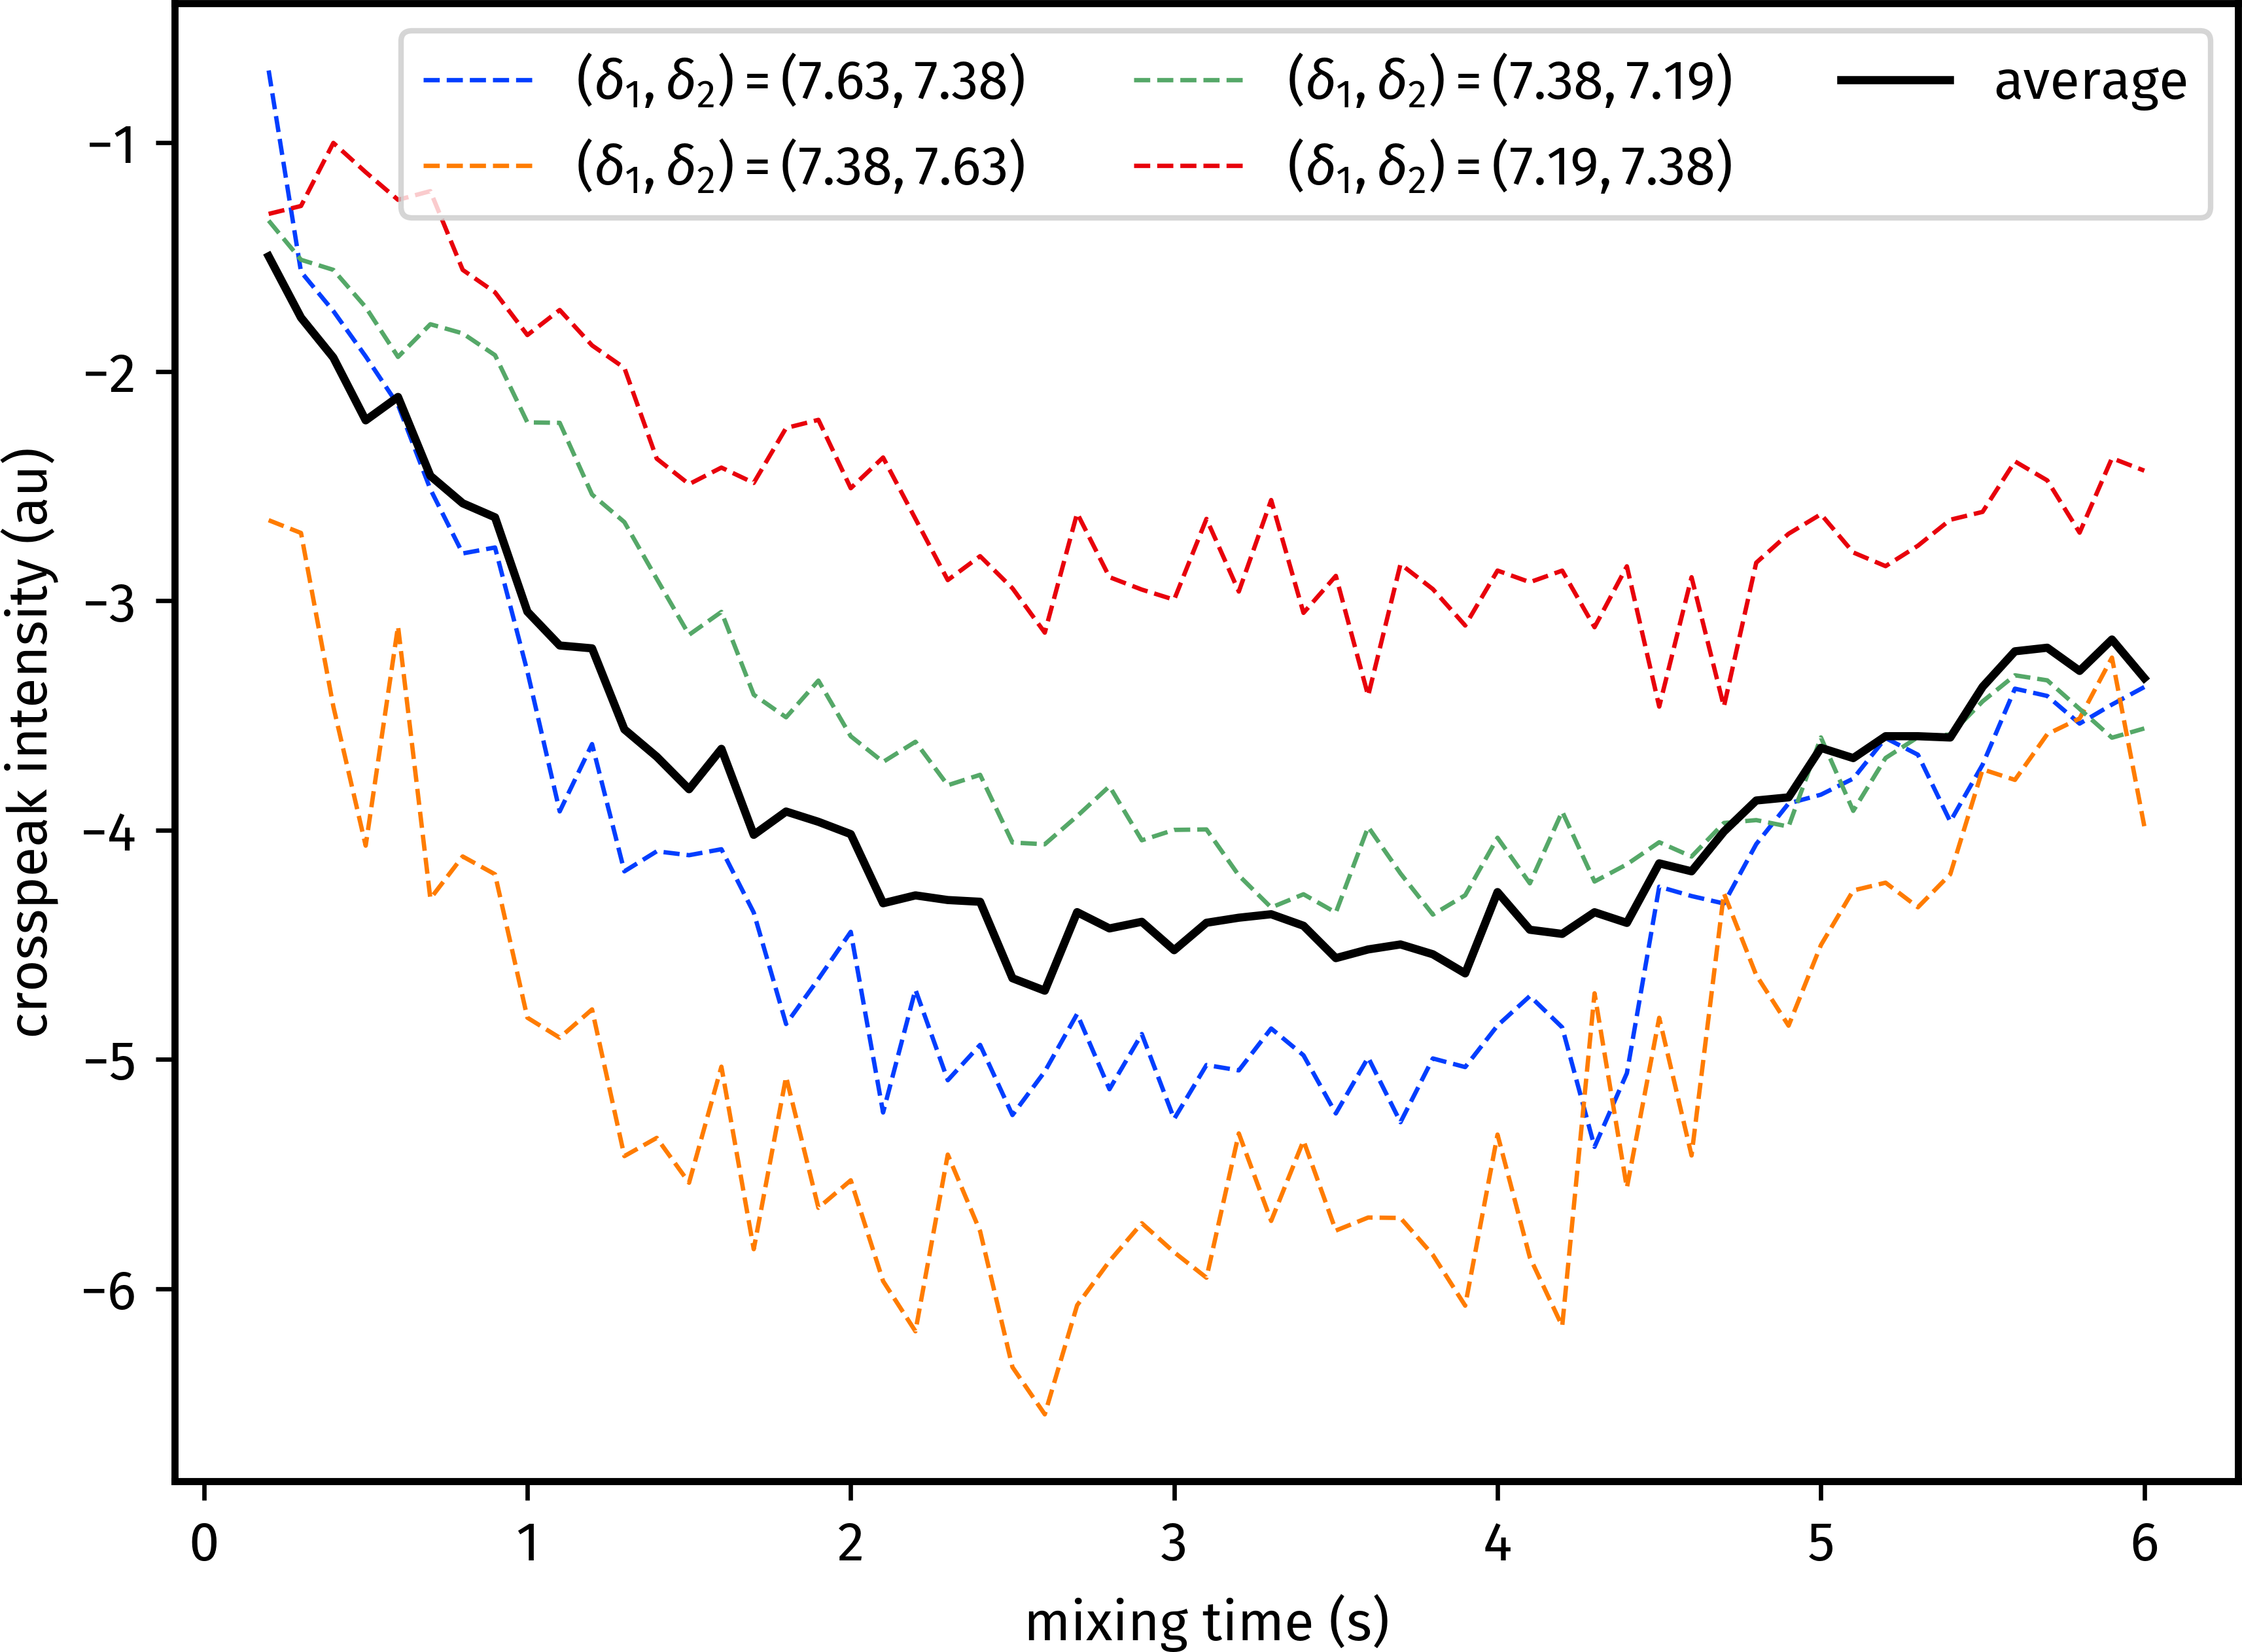
\includegraphics[draft=false]{poise/noesy_scan.png}
    \caption[Scan of 2D NOE crosspeak intensities]{
        Scan of 2D NOE crosspeak intensities.
        The individual crosspeak intensities are shown in dashed lines; the solid black line is the average of these four, which represents the quantity we seek to optimise.
        \datacode{7B-200725}
    }
    \label{fig:poise_noesy_scan}
\end{figure}

In the chosen sample, 3-fluorophenylboronic acid, there are four crosspeaks of interest in the 2D NOESY spectrum.
I first scanned over a range of mixing times to determine where the crosspeak intensities were maximised (\cref{fig:poise_noesy_scan}).
Generally, a broad minimum between 2.5 and \SI{4}{\s} is observed: any result within this range should be considered as `correct'.%
\footnote{There is a complicating factor in that the use of such long mixing times also leads to a noticeable increase in the experiment duration. As such, it is not necessarily the case that an optimised mixing time yields a greater sensitivity \textit{per unit time}. In the optimisations which follow, I have neglected this issue. However, it could probably be somewhat accounted for by modifying the form of the cost function.}
Although this may at first glance seem imprecise, it merely reflects the underlying physical characteristics of the sample under study: it is not the job of an optimisation process to `discover' extra precision where there is none to be found.
We also see here the first example of a cost function where the noise is significant: this provides a good test of the derivative-free algorithms used in POISE.

While the 2D NOESY scan offers first-hand insight into what our target optimum should be, it is unwise to run an optimisation using the full 2D experiment, simply because of the time required for each FE.
A more sensible method is to use a selective 1D NOESY experiment, where the mixing time is represented by the parameter \texttt{D8}.
Although this is much faster, it does come with two caveats:
\begin{enumerate}
    \item The frequency for selective irradiation must be first chosen, likely after acquisition of a 1D \proton{} spectrum.
        Thus, the optimisation does require some \textit{a priori} knowledge of the system being studied.
    \item The crosspeak intensities in the 1D NOESY \textit{must} be sufficiently representative of those in the full 2D NOESY.
\end{enumerate}

The cost function used (\texttt{noe\_1d}) must thus pick out only the crosspeaks from the 1D NOESY spectrum.
It does this by detecting the frequency used for the selective irradiation (which is given by the \texttt{SPOFFS2} parameter), excising a region of ca.\ \SI{100}{\Hz} around the irradiation frequency, and integrating the remainder of the spectrum.
In order to account for the fact that the NOE crosspeaks may be either positive or negative (depending not only on the molecular weight, but also how the spectrum is phased), the absolute value of the integral is taken, and the negative of this is used as the cost function (since we seek to maximise the intensity).
Note that if a different 1D NOESY pulse programme is used with different parameter definitions, then the cost function must be adjusted accordingly.

\begin{figure}[htb]
    \centering
    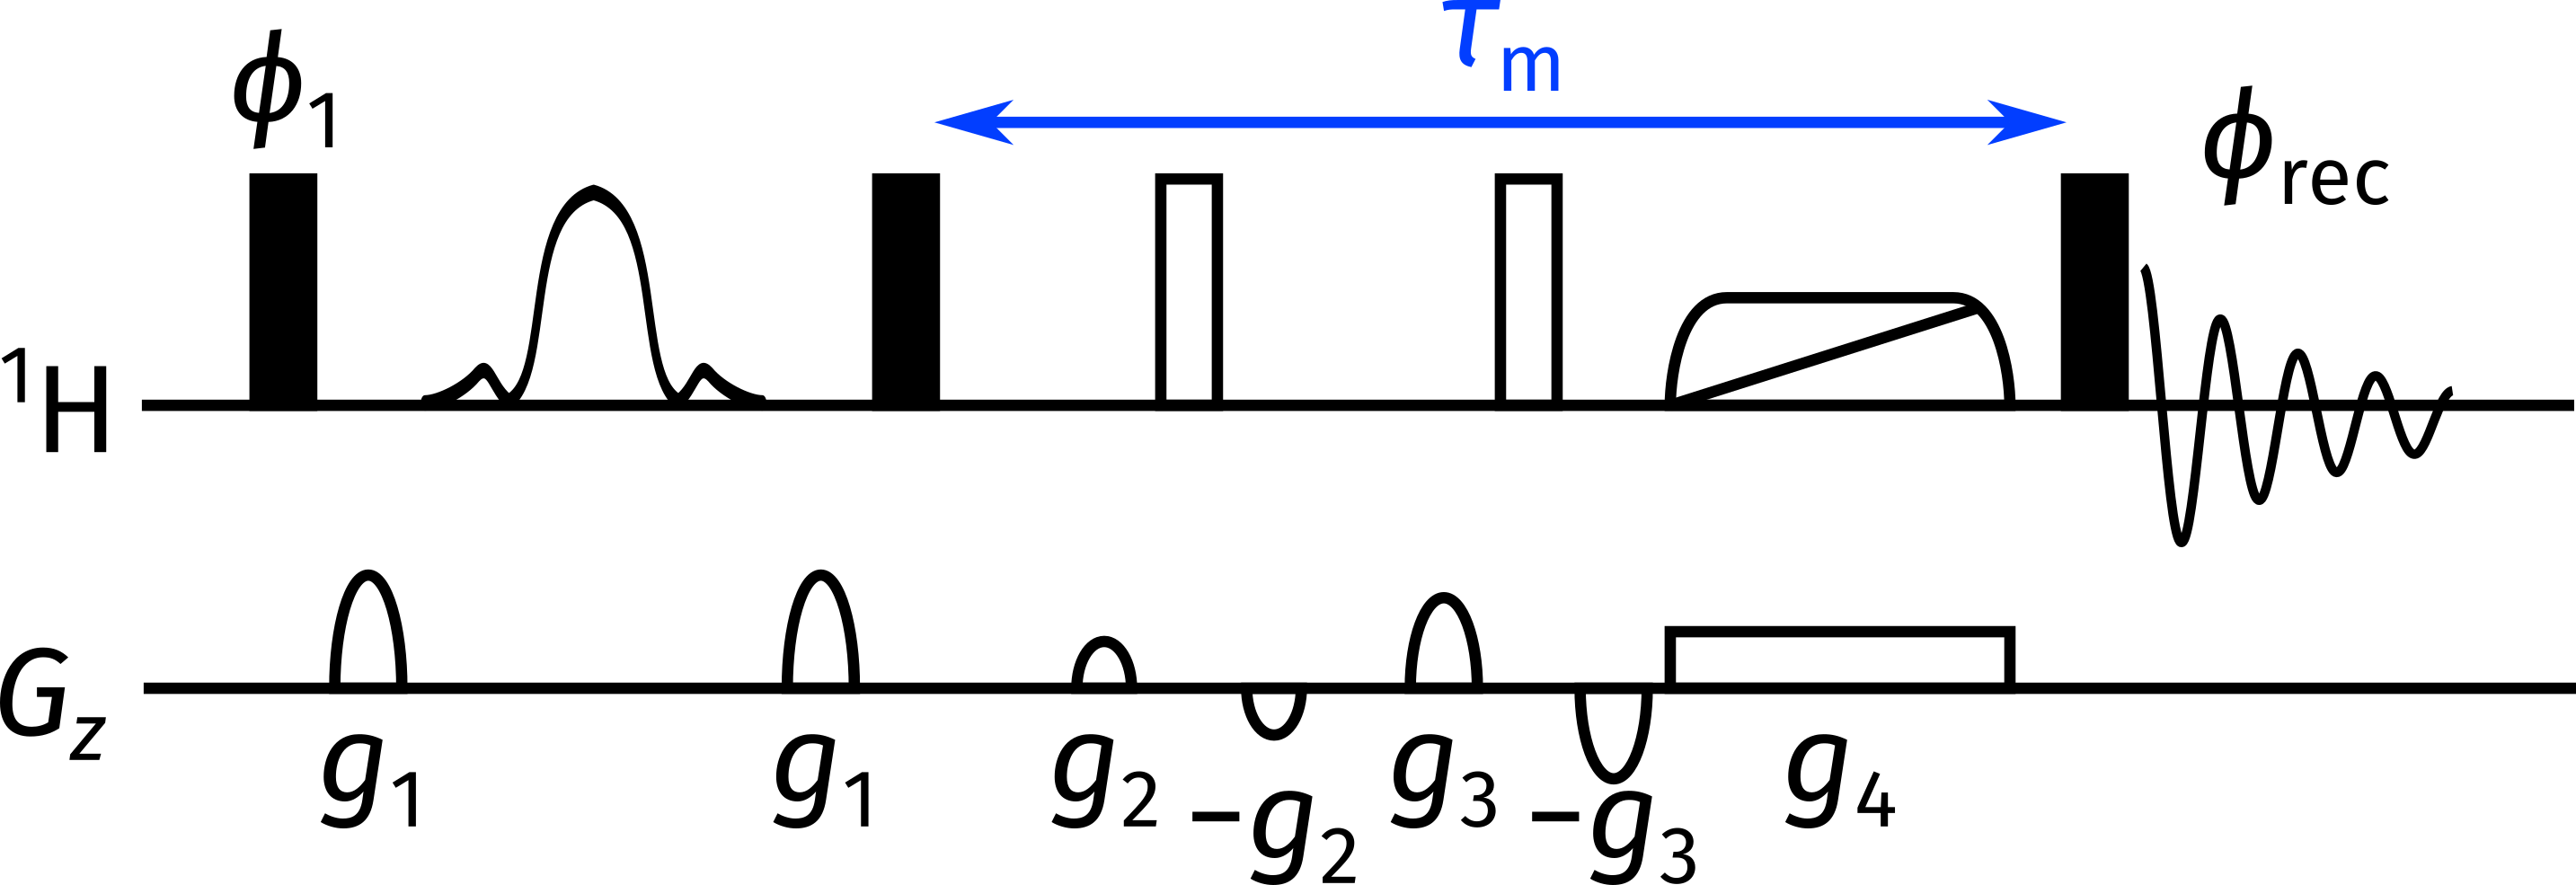
\includegraphics[draft=false]{pp/poise/noe1d.png}
    \caption[1D NOESY pulse sequence used for POISE optimisations]{
        Selective 1D NOESY pulse sequence used for POISE optimisations.
        Phase cycling was performed using $\phi_1 = \phi_\text{rec} = (x, -x)$.
        The exact gradient amplitudes used are not hugely important, except for the $z$-filter gradient $g_4$, which should be calibrated as per the protocol in Thrippleton et al.\autocite{Thrippleton2003ACIE}
    }
    \label{fig:noe1d_pulseq}
\end{figure}

In the event, I used a modified 1D NOESY pulse programme (\cref{fig:noe1d_pulseq}), with two extra inversion pulses during the mixing time: these minimise artefacts arising from relaxation during the mixing time, which can be especially problematic for long mixing times of several seconds.
(In principle, these artefacts have equal positive and negative components and thus should not contribute to the cost function except in terms of noise; however, it is always a good idea to minimise the noise in the cost function as much as possible.)
The initial value for the optimisation was set to \SI{0.5}{\s}, which is a reasonable compromise value for most `small' organic molecules.

\subsubsection{Optimisation results}

\begin{table}[htb]
    \hbadness=10000
    \centering
    \begin{tabular}{ccccc}
        \toprule
        Entry & Algorithm & Optimum found (\si{\s}) & FEs    & Time taken (\si{\s}) \\
        \midrule
        1     & NM        & 3.25--3.88              & 16--18 & 268--312             \\
        2     & MDS       & 3.63--3.75              & 16--18 & 269--305             \\
        3     & BOBYQA    & 3.38--3.80              & 6--10  & 88--162              \\
        \bottomrule
    \end{tabular}
    \caption[NOE mixing time optimisations on 3-fluorophenylboronic acid]{
        NOE mixing time optimisations on a sample of 3-fluorophenylboronic acid.
        The POISE routine used here is: \mintinline[breaklines]{json}{{"name": "1dnoe", "pars": ["d8"], "lb": [0.2], "ub": [6.0], "init": [0.5], "tol": [0.1], "cf": "noe_1d", "au": "poise_1d"}}.
        \datacode{7B-200721}
    }
    \label{tbl:poise_noe_3fpba}
\end{table}

The results of this optimisation are shown in \cref{tbl:poise_noe_3fpba}.
In all cases, the optimisations converged to the correct region within 2.5 minutes (for BOBYQA) and 5 minutes (for the simplex-based algorithms).
The resulting 2D NOESY spectra, with the initial and optimised mixing times of \SI{0.5}{\s} and \SI{3.5}{\s} respectively, are shown in \cref{fig:poise_noesy}, where the improvement in crosspeak sensitivity is clearly visible.

\begin{figure}[htb]
    \centering
    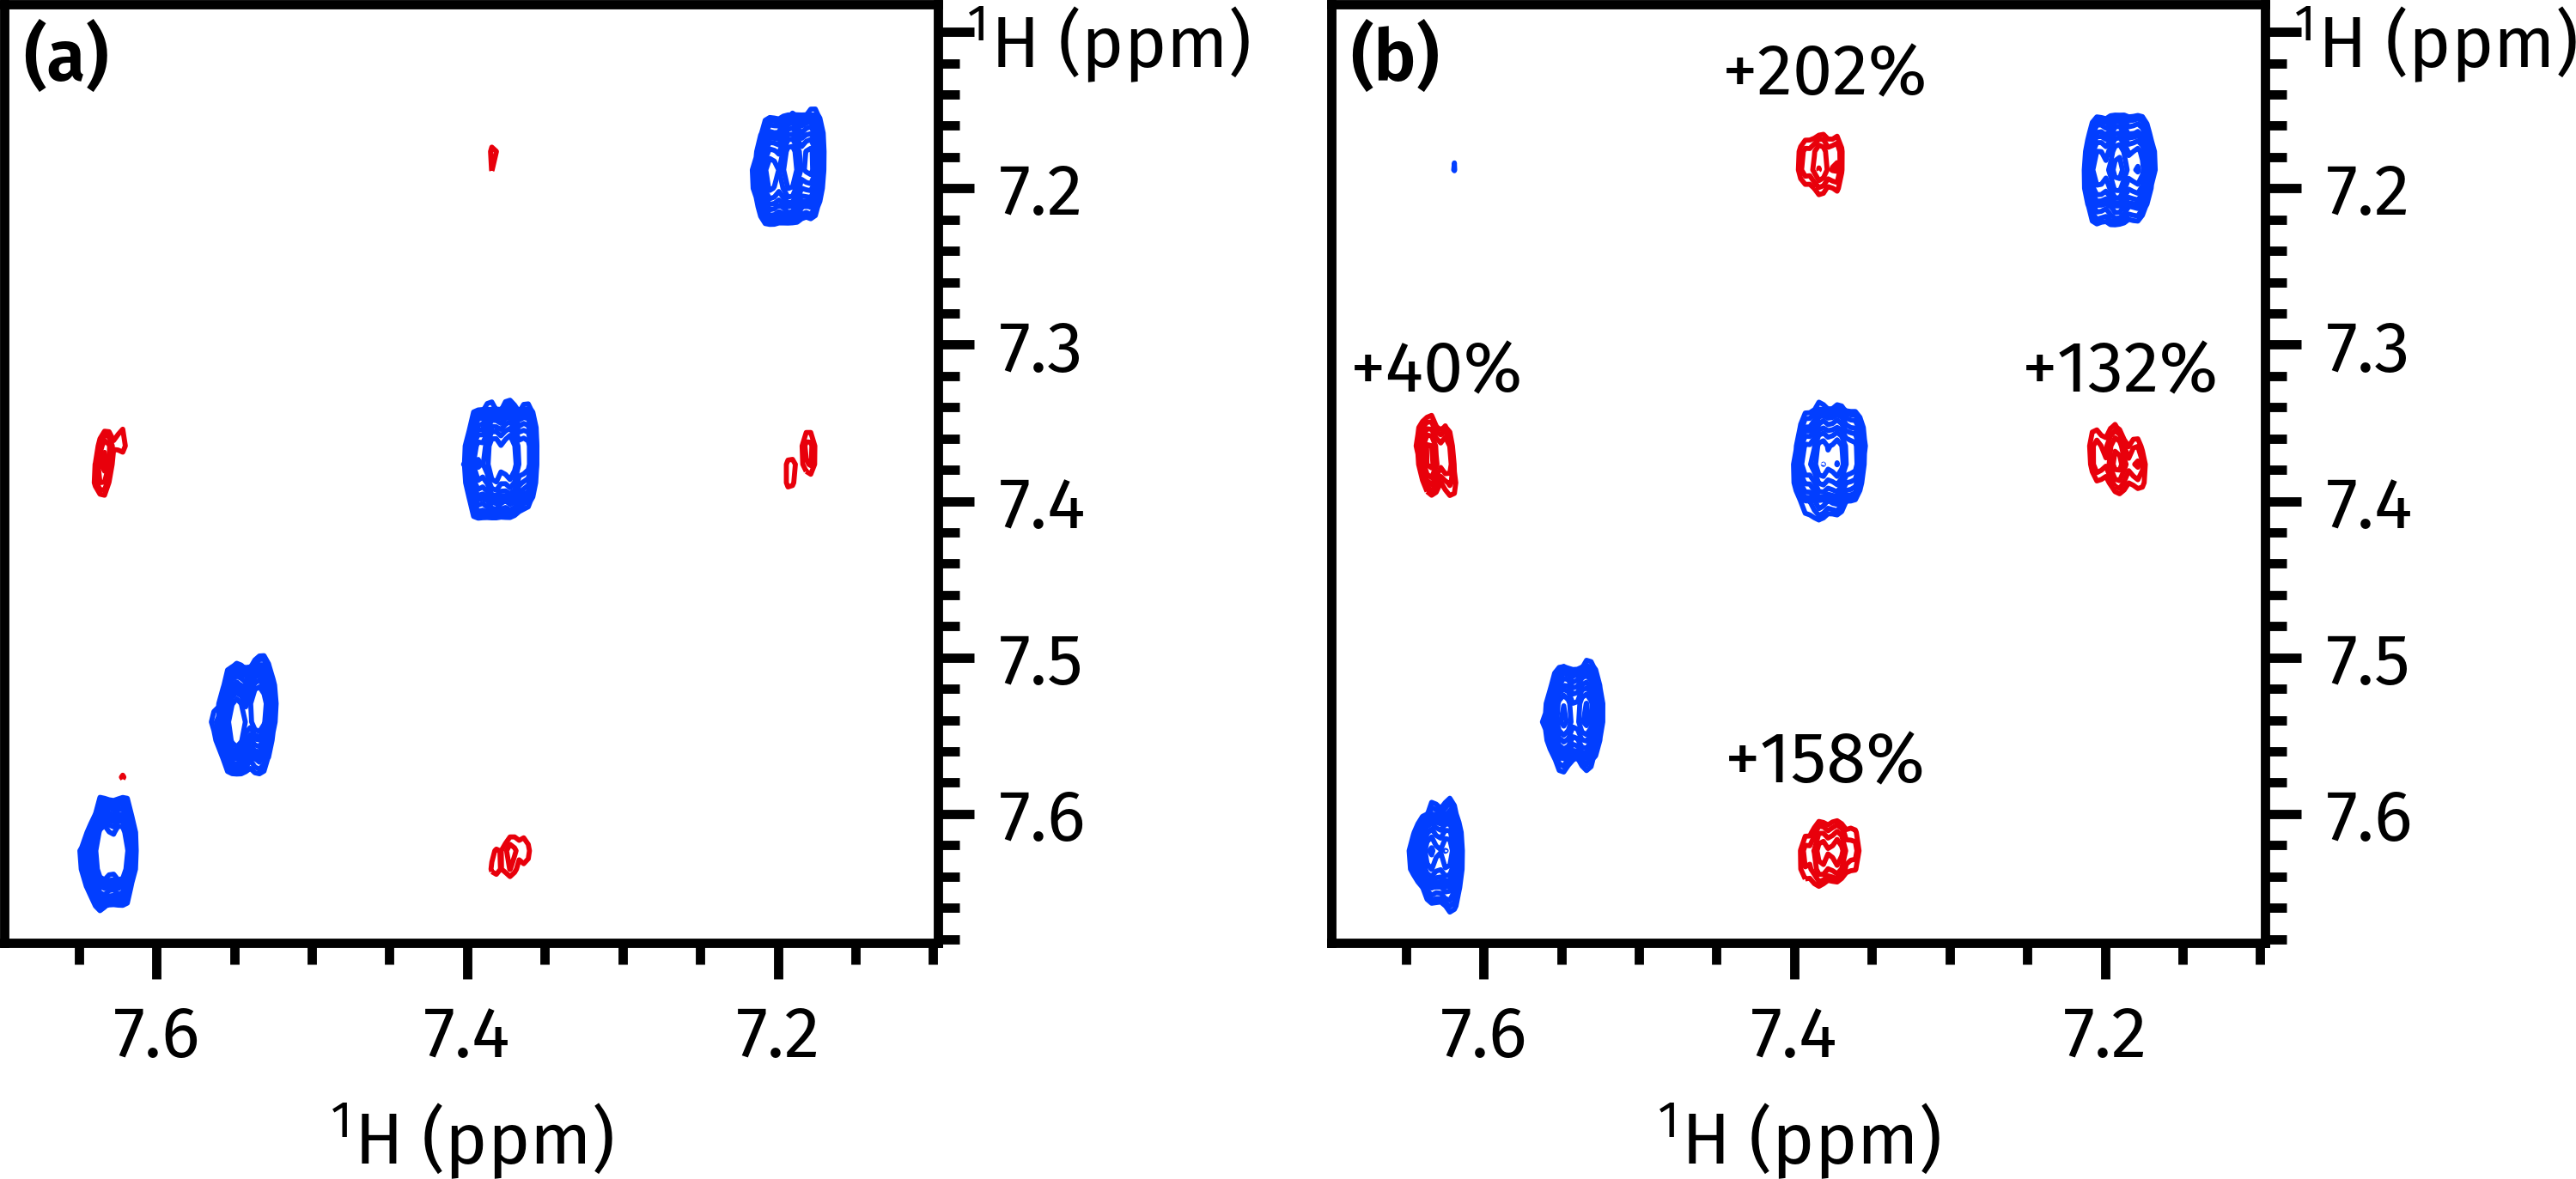
\includegraphics[draft=false]{poise/noesy_spec.png}
    {\phantomsubcaption\label{fig:poise_noesy_unoptimised}}
    {\phantomsubcaption\label{fig:poise_noesy_optimised}}
    \caption[2D NOESY spectra before and after optimisation]{
        2D NOESY spectra of 3-fluorophenylboronic acid, obtained 
        \textbf{(\subref{fig:poise_noesy_unoptimised})} before and 
        \textbf{(\subref{fig:poise_noesy_optimised})} after optimising the mixing time on the 1D NOESY sequence in \cref{fig:noe1d_pulseq}.
        Both spectra are plotted with the same contour levels.
        \datacode{7B-200725}
    }
    \label{fig:poise_noesy}
\end{figure}

It should be mentioned here that each FE was run using one dummy scan and two scans.
This was made possible due to the high SNR afforded by a concentrated sample (\SI{120}{\milli\molar}), as well as a cryogenic probe.
For more dilute samples where SNR is insufficient, the POISE optimisation will require more scans per FE, and consequently will take longer.
However, it can be argued that the \textit{benefit} reaped from the optimisation is also correspondingly larger, since the final (optimised) 2D NOESY which is run will also take a longer time.


\subsubsection{A different sample}

To more clearly illustrate the \textit{sample-specific} nature of POISE optimisations, it is also useful to run the same optimisation on a different sample: in this case, the decapeptide gramicidin S.
For this rather larger compound, we would expect the optimisation to converge instead to a shorter mixing time, and this is validated in practice (\cref{tbl:poise_noe_grami}).
The peak at \SI{4.76}{\ppm} was used for selective irradiation: this is the \ch{H}$^{\alpha}$ proton of the ornithine residue.

\begin{table}[htb]
    \hbadness=10000
    \centering
    \begin{tabular}{ccccc}
        \toprule
        Entry & Algorithm & Optimum found (\si{\s}) & FEs    & Time taken (\si{\s}) \\
        \midrule
        1     & NM        & 0.63--0.78              & 9--14  & 253--384             \\
        2     & MDS       & 0.44--0.75              & 9--11  & 254--309             \\
        3     & BOBYQA    & 0.58--0.77              & 5--8   & 136--223             \\
        \bottomrule
    \end{tabular}
    \caption[NOE mixing time optimisations on gramicidin]{
        NOE mixing time optimisations on a sample of gramicidin S.
        The POISE routine used here is identical to before.
        \datacode{7G-210815}
    }
    \label{tbl:poise_noe_grami}
\end{table}
